\section{Run-Time Assurance}
\label{sec:rta}

%Moved description of plan selector and decision logic table to the end of this section

Run-time assurance architectures add high-assurance components
to the system to ensure that a complex or difficult-to-verify component (such as our LEC) cannot cause
unsafe or unintended system behaviors. Run-time monitors
continuously check input or output values of the LEC to assess safety and can intervene to
switch to a backup function that is proven to be safe. 

In this project Collins Aerospace engineers developed a
run-time assurance architecture based on the ASTM F3269-17
standard for bounded behavior of complex systems \cite{F3269-17}, also
known as a simplex architecture \cite{simplex}. The standard provides
guidance for mitigating unintended behaviors through the
use of run-time monitors. The LEC may still produce unintended
behavior, but the architecture ensures that there will
be no impact on system safety. This approach  uses
the verified properties of the architecture, run-time monitor,
and safety backup function to justify a reduced level of
criticality for the LEC.

The run-time assurance architecture is illustrated in the green box in Figure~\ref{fig:rta-arch}.  Incoming ADS-B messages are assessed by the DAA subsystem.  When an avoidance alert is generated, the Backup Avoidance Planner and the LEC Planner both generate avoidance flight plans.  The RTA monitors perform a ``remain well clear'' (RWC) assessment on both plans, determining whether either plan will result in a violation of the DO-365 separation requirements.  Based on the assessments, Plan Selector then chooses one of the two plans and the Plan Switch publishes the chosen flight plan.

\subsection{Trajectory Prediction} 
Trajectory prediction over a defined prediction horizon (in time units) consists of prediction of both the intruder and own-ship trajectories based on underlying assumptions of the intruder's future velocity and the own-ship's ability to track the avoidance flight plans from the LEC and the Safe Backup Planner. For the application in consideration, the prediction horizon was set to 180 seconds under the assumption that the avoidance flight plans produced would be frozen for this time period. In cases where the avoidance plans can be generated more frequently, the prediction horizon can appropriately be reduced which should improve the accuracy of intruder trajectory prediction and allow for more confidence in the RWC evaluation.

For the intruder, each incoming ADS-B message is processed as a measurement to a tracking filter designed as per Appendix D in \cite{DO_366A}. The tracking filter assumes that the intruder aircraft is either in a constant velocity (CV) mode or in a constant speed turn (CT) mode. The multiple-model tracking filter is designed to be robust to basic errors in the ADS-B message data (such as data with too small or large uncertainties), missing data or repeat data, but mostly the ADS-B data is considered a trustworthy source of information of the intruder 3D position. The tracking filter produces estimates of the intruder current position and velocity along with their respective uncertainties, and with a prediction of the specific mode of the intruder behavior (CV/CT). The trajectory prediction propagates the estimate from the tracking filter forward in time by assuming the aircraft continues in its current mode (CV/CT) with a growth model in the longitudinal velocity uncertainty and a cross-track position uncertainty, with the cross-track position uncertainty capped to a maximum value. The uncertainties in the intruder trajectories can be visualized as ellipses whose semi-major/semi-minor axes are aligned with the longitudinal/normal to velocity vector and whose lengths are proportional to the uncertainties along/normal to the velocity vector. These assumptions allow to account for decaying confidence over longer prediction horizons.

The own-ship trajectory predictions along the avoidance flight plans assume a kinematic model of the own-ship behavior using performance parameters such as maximum bank angle, roll-rate, longitudinal acceleration, etc. The trajectory prediction assumes that the first waypoint of the avoidance flight plans lies directly in the path of the current velocity vector. The own-ship trajectory consists of constant ground speed segments between waypoints and constant speed arcs connecting line segments between consecutive waypoints. As the actual aircraft is flying at a constant airspeed, and not ground speed, deviations between the predicted and actual aircraft trajectories are expected. These deviations are accounted for by a fixed tracking error bound that is configurable. The tracking error bound and vehicle size parameter are added to the specified RWC separation distance to produce a conflict radius threshold around the own-ship.

The trajectory prediction models are run internally at a high-rate (over 10 Hz) for both the intruder and own-ship, but the output trajectories are sampled at 1 Hz to produce time-stamped discretized trajectory points which are evaluated for conflicts as discussed in the next sub-section.

\subsection{Remain Well Clear Assessment} 
The RWC assessment consists of evaluating time-stamped samples of the predicted trajectory of the intruder and the own-aircraft trajectory along each produced avoidance flight plan. The evaluation considers the intersection of the uncertainty ellipse around an intruder predicted trajectory sample with the conflict circle around the corresponding own-ship predicted trajectory sample. The probability of intersection is determined using the analytical approximations documented in Section IV of \cite{prob_conflict_detection}. If the probability exceeds a configurable threshold, then the flight plan is determined to be unsafe. 

In addition to the determination of safety, the closest point of approach (CPA) between the own-ship and intruder predicted trajectories is calculated along with the time to CPA. The CPA metrics allow the Plan Selector decision logic component to choose between plans that are both marked unsafe by the RWC assessment. These metrics allow for a comparison with the actual measured CPA metrics during simulation and test flights as a way to evaluate the run-time monitor performance.

\subsection{Plan Selector}

% [ERIC/KARTHIK - 1 pg]

% Decision logic, tabular spec and evolution, APT synth and proof \\

% might want to cite Alessandro's recent APT/ATJ/ATC papers?

A critical component of the RTA architecture is the Plan Selector, which selects the flight
plan to be used based on formally verified decision logic. This decision logic specifies the rules
that determine whether the LEC flight plan or the Backup Avoidance flight plan (BAF) should
be selected based on the results received from the RWC Assessment component. The
decision logic is specified in a tabular format, shown in Figure~\ref{fig:selection-logic}.
After running the logic, the Plan Selector sends its decision to the
aircraft Plan Switch.

When a flight plan assessment is received, it is evaluated based on five
variables, including the RWC metrics:  plan validity (whether a plan has been received), plan
safety, whether the time of closest point of approach (tCPA) is greater than
179 seconds (the end of the planning horizon), comparison of the predicted miss
distance (pmd) between the intruder and own-ship, and whether three seconds has elapsed since the
receipt of the first plan.

If only one plan has been received by the three second timeout, we select (publish)
that plan by default.
If we receive two plans and only one is safe, we select the safe plan.
If neither plan is safe, we select the one with the larger predicted miss distance.
If both plans are safe, the LEC plan is usually selected.  However, there is some
additional tie-breaking logic.
If tCPA is beyond the planning horizon for one of the plan, this means that we don't really know what
its true CPA is so we select the other plan.
If tCPA is beyond the planning horizon for both plans, we fall back to selecting the plan with
the greater predicted miss distance.

Different selection logic could be specified depending on vehicle and program requirements,
and indeed our specification evolved over the course of the project.  However, the
formal synthesis approach (described in the next section) ensures that we can
quickly regenerate a correct implementation of the specification.

%not valid, we deem it unfit for publication.  If a plan is valid, and we've yet
%to receive the other plan after 3 seconds, we go ahead and publish the plan we
%received.  Otherwise, we've received two valid plans.  If exactly one of them
%is safe, we publish it.  If neither plan is safe, we publish the one with the
%larger predicted miss distance.
%Otherwise, both plans are safe, so we consider
%whether their times of closest approach are beyond the 179 second limit.  If
%exactly one plan's tCPA is beyond the limit, we choose the other plan.  If
%neither is beyond the limit, we chose the LEC plan.  Otherwise, both plans'
%tCPA is beyond the 179 second limit.  In that case, we choose the plan with the
%larger predicted miss distance.  See Figure~\ref{fig:selection-logic} for the
%full decision table.

\begin{figure*}
	\centering
	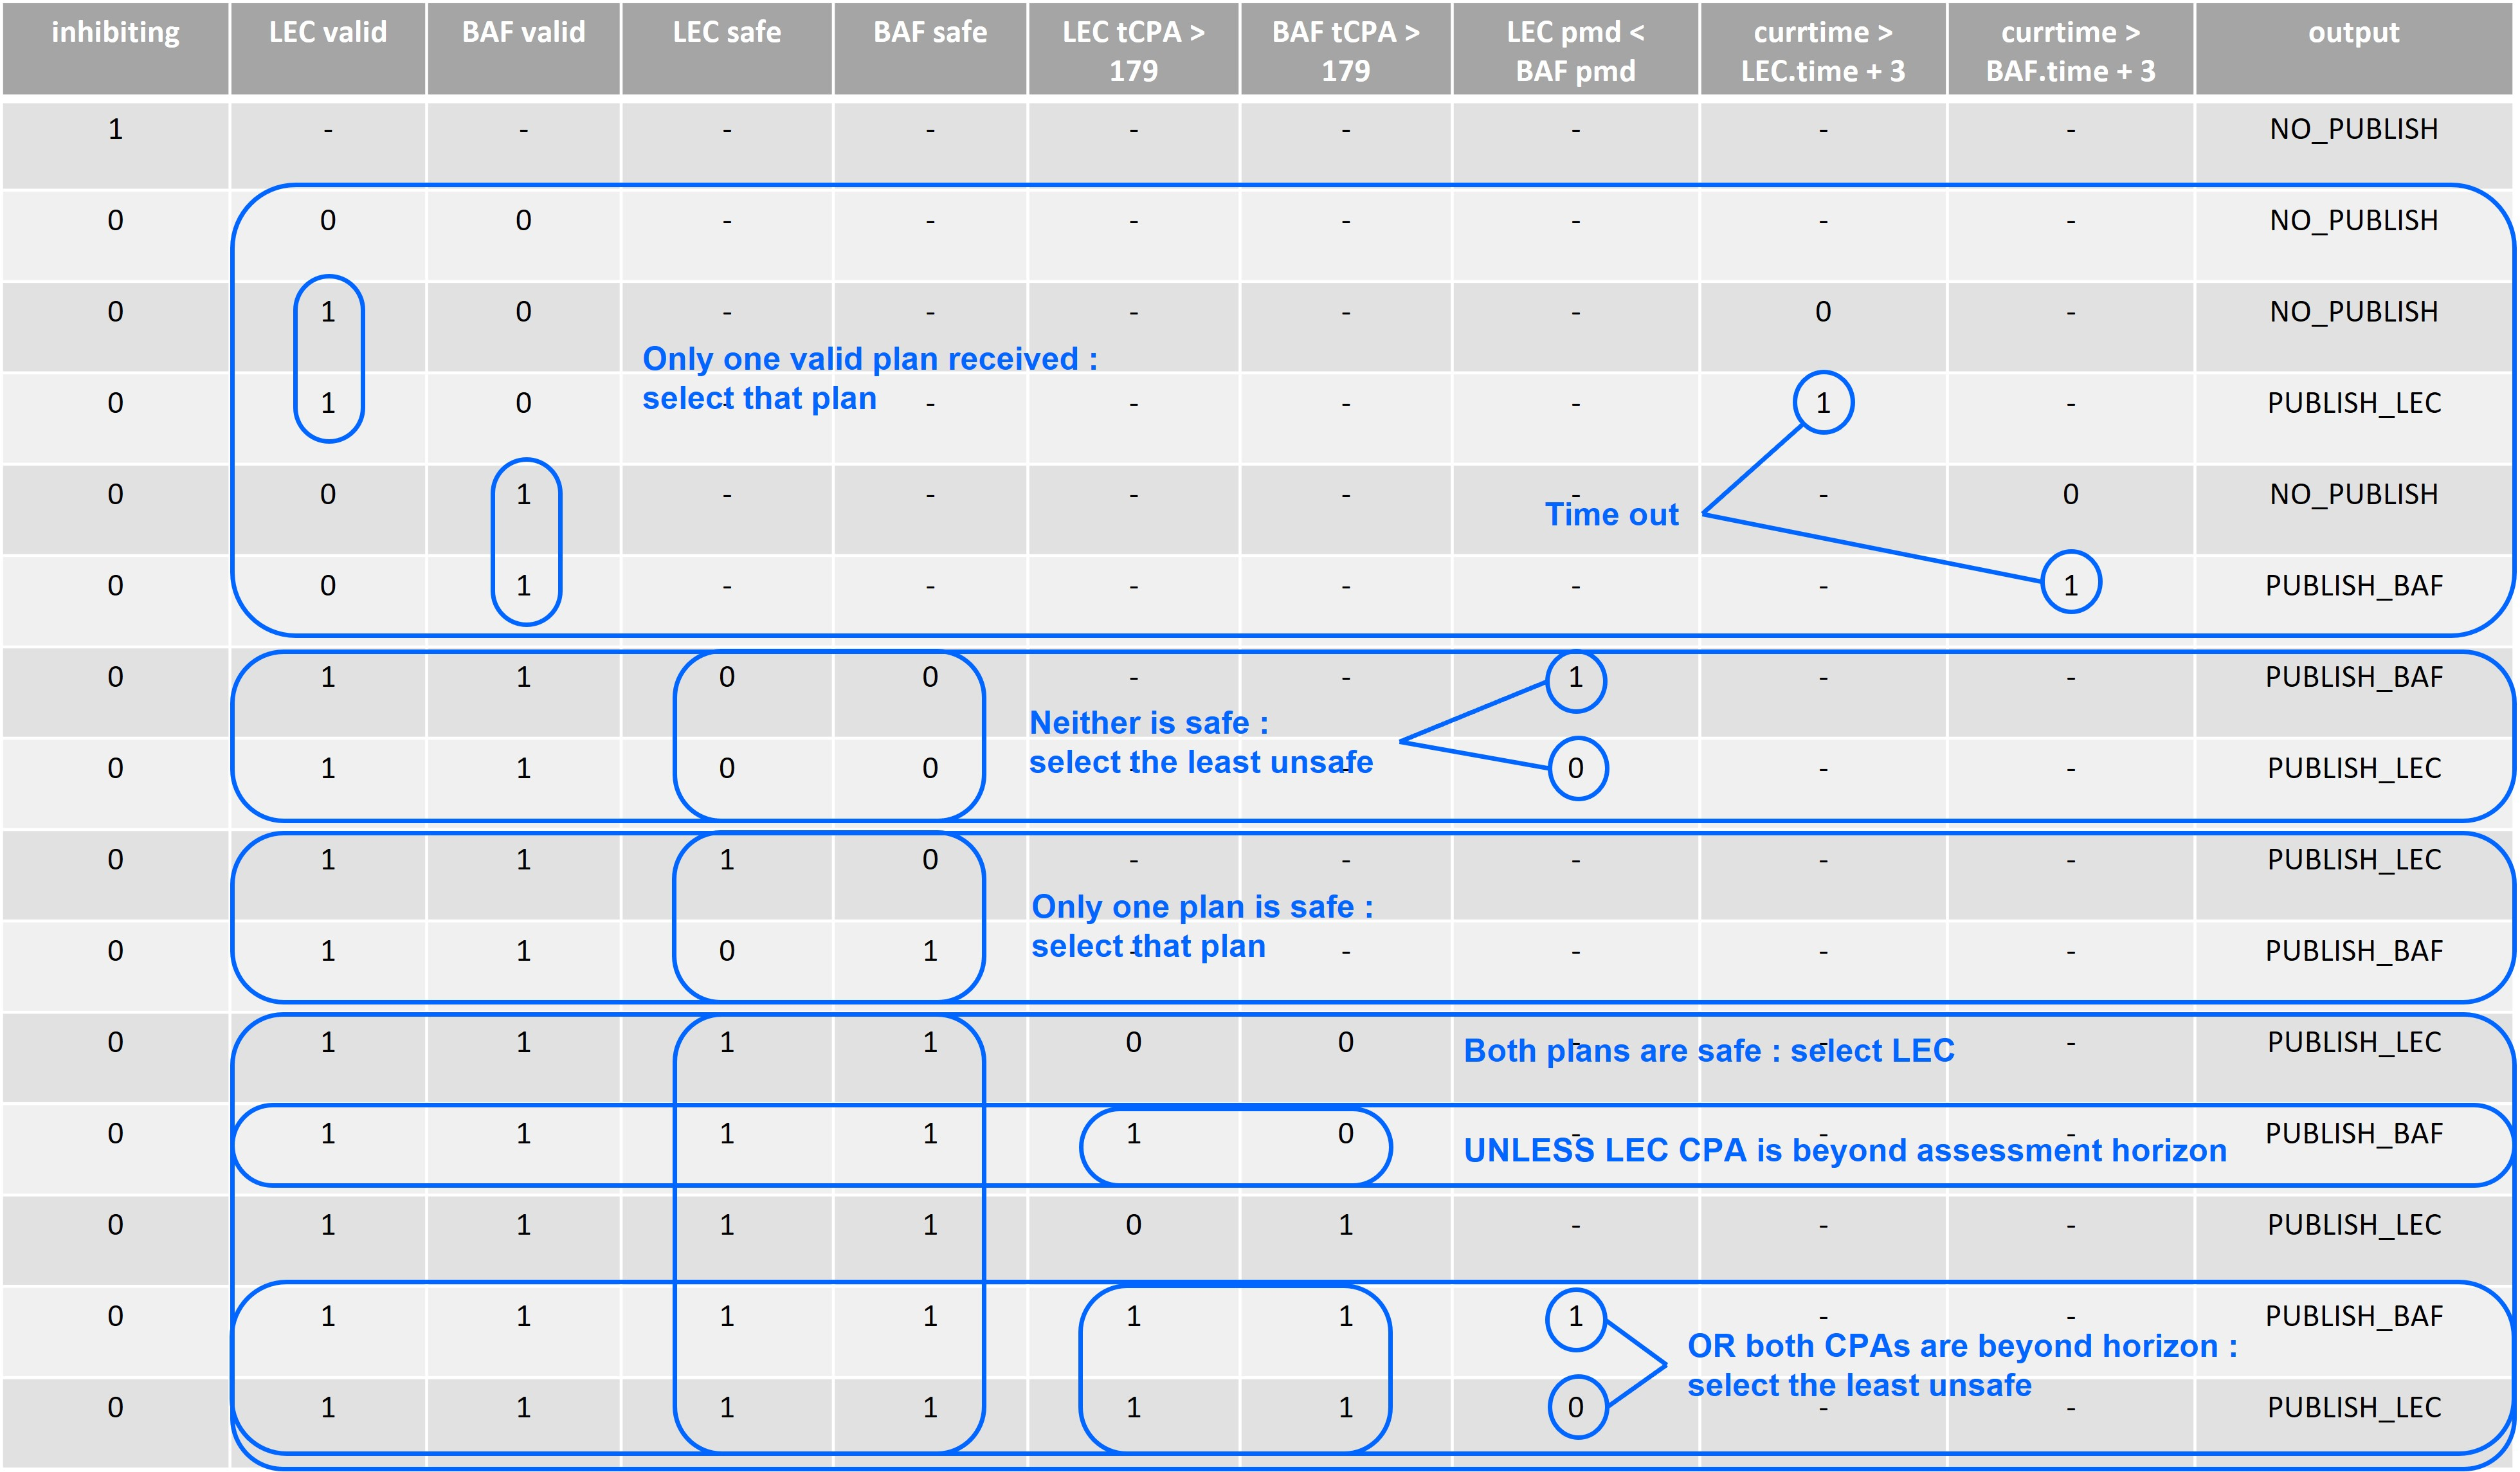
\includegraphics[width=\textwidth]{figures/selection-logic.jpg}
	\caption{Plan Selection logic specification (hyphens match either 0 or 1)}
	\label{fig:selection-logic}
\end{figure*}

